\documentclass[10pt,a4paper]{article}

\usepackage[utf8]{inputenc}
\usepackage[T1]{fontenc}
\usepackage[spanish,es-nodecimaldot]{babel}
\usepackage[top=1.5cm, bottom=2cm, left=1.5cm, right=1.5cm]{geometry}
\usepackage{setspace}
\singlespacing
\usepackage{graphicx}
\usepackage{float}
\usepackage{booktabs}
\usepackage{array}
\usepackage{tabularx}
\usepackage{hyperref}
\usepackage{xcolor}
\usepackage{amsmath}
\usepackage{caption}
\usepackage{listings}
\usepackage{parskip}
\usepackage[numbers]{natbib}
\usepackage{fancyhdr}

\definecolor{codebackground}{HTML}{F5F5F5}
\definecolor{codecomment}{HTML}{6A9955}
\definecolor{codestring}{HTML}{CE9178}
\definecolor{codekeyword}{HTML}{569CD6}
\definecolor{headerdark}{HTML}{2C3E50}

\lstset{
  language=R,
  backgroundcolor=\color{codebackground},
  basicstyle=\ttfamily\footnotesize,
  breaklines=true,
  frame=single,
  rulecolor=\color{gray!40},
  commentstyle=\color{codecomment},
  stringstyle=\color{codestring},
  keywordstyle=\color{codekeyword}\bfseries,
  numbers=left,
  numberstyle=\tiny\color{gray},
  numbersep=5pt,
  tabsize=2,
  showstringspaces=false,
  captionpos=b
}

\hypersetup{
  colorlinks=true,
  linkcolor=headerdark,
  citecolor=headerdark,
  urlcolor=blue!70!black,
  pdftitle={Analisis de Componentes Principales del Dataset Boston},
  pdfauthor={Vicente Rivera, Juan Munoz, Fernando Valdes}
}

\captionsetup{font=small, labelfont=bf}

\begin{document}

\begin{center}
  {\large \textbf{Universidad Catolica de Temuco}} \\[2pt]
  {\normalsize Facultad de Ingenieria -- INFO1184 Inteligencia de Negocios} \\[8pt]
  \rule{0.86\textwidth}{0.6pt} \\[8pt]
  {\Large \textbf{TAREA 04}} \\[4pt]
  {\LARGE \textbf{Analisis de Componentes Principales}} \\[4pt]
  {\LARGE \textbf{Dataset Boston -- Metodologia CRISP-DM}} \\[10pt]
  {\normalsize \textbf{Docente:} Marcos Levano Humacto} \\[3pt]
  {\normalsize \textbf{Desarrollado por:} Vicente Rivera, Juan Mu\~noz, Fernando Valdes} \\[2pt]
  {\small vrivera2023@alu.uct.cl, juan.munozveloso2023@alu.uct.cl, fvaldes2023@alu.uct.cl} \\[2pt]
  {\small Tarea 4, INFO1184, Semestre I-2026} \\[8pt]
  \rule{0.86\textwidth}{0.6pt}
\end{center}

\section*{Resumen}

El presente informe desarrolla un analisis de datos y visualizacion del dataset \texttt{Boston}, disponible en el paquete \texttt{MASS} de R, mediante la tecnica central de Analisis de Componentes Principales (PCA). El trabajo sigue la metodologia CRISP-DM en sus fases de comprension del negocio, comprension de los datos, preparacion, modelamiento y evaluacion. El conjunto contiene 506 observaciones y 14 variables asociadas a criminalidad, caracteristicas urbanas, accesibilidad, contaminacion, condicion socioeconomica y valor mediano de viviendas. Se detectaron valores atipicos mediante la regla del rango intercuartil, se analizaron relaciones entre precio, habitaciones, condicion de limitar con el rio Charles y estatus socioeconomico, y se uso PCA para sintetizar la estructura multivariada que respalda esas relaciones. Los cinco primeros componentes explicaron el 80,58\% de la varianza total. Adicionalmente, se entreno una regresion lineal sobre componentes principales para predecir \texttt{log1p(crim)}, obteniendo un $R^2$ de 0,8119 en escala logaritmica y una mejora de 11,85\% en RMSE frente al promedio base. El analisis confirma patrones relevantes para interpretar el valor habitacional y la criminalidad en el caso Boston.

\textbf{Palabras clave:} PCA, CRISP-DM, Boston, vivienda, criminalidad, R Project.

\section{Introduccion}

La inteligencia de negocios aplicada al analisis urbano permite transformar datos historicos en informacion util para comprender precios de viviendas, condiciones del entorno y riesgos territoriales. El dataset \texttt{Boston} recopila informacion de suburbios del area de Boston, con variables relacionadas con criminalidad, uso de suelo, contaminacion, accesibilidad, educacion, estatus socioeconomico y precio mediano de viviendas.

El objetivo de esta tarea es aplicar Analisis de Componentes Principales (PCA) siguiendo CRISP-DM para responder seis preguntas de investigacion: (1) si existen valores atipicos en al menos dos variables; (2) que suburbios tienen las casas mas baratas; (3) como influye el tamano de la casa en su precio; (4) si la condicion de limitar con el rio Charles afecta el valor; (5) cual es el impacto del estatus socioeconomico; y (6) si es posible predecir la tasa de criminalidad. El desarrollo fue implementado en R, usando codigo simple y reproducible.

\section{Fundamentos de Teoria}

\subsection{Metodologia CRISP-DM}

CRISP-DM (\textit{Cross-Industry Standard Process for Data Mining}) es una metodologia ampliamente usada para ordenar proyectos de mineria de datos. Sus fases son: comprension del negocio, comprension de los datos, preparacion de los datos, modelamiento, evaluacion y despliegue \citep{chapman2000}. En esta tarea se desarrollan las fases 1 a 5, tal como indica el enunciado.

\subsection{Analisis de Componentes Principales}

El Analisis de Componentes Principales transforma un conjunto de variables posiblemente correlacionadas en nuevas variables no correlacionadas llamadas componentes principales \citep{jolliffe2002}. Cada componente es una combinacion lineal de las variables originales y se ordena segun la cantidad de varianza explicada. Si $x_1, x_2, \ldots, x_p$ son variables estandarizadas, un componente se puede expresar como:

\begin{equation}
  PC_k = a_{1k}x_1 + a_{2k}x_2 + \cdots + a_{pk}x_p
\end{equation}

donde $a_{jk}$ corresponde a la carga de la variable $j$ en el componente $k$. Como las variables tienen escalas distintas, se uso estandarizacion \textit{z-score}:

\begin{equation}
  z = \frac{x - \bar{x}}{s_x}
\end{equation}

donde $\bar{x}$ es la media y $s_x$ la desviacion estandar. Esta transformacion evita que variables con rangos grandes dominen el PCA.

\subsection{Regresion con Componentes Principales}

Para evaluar si es posible predecir la criminalidad, se uso regresion lineal sobre componentes principales. Esta estrategia reduce colinealidad entre predictores porque los componentes son ortogonales. La variable objetivo fue transformada como \texttt{log1p(crim)} para reducir la asimetria y el efecto de valores extremos. El desempeno se evaluo con RMSE, MAE y $R^2$:

\begin{equation}
  RMSE = \sqrt{\frac{1}{n}\sum_{i=1}^{n}(y_i - \hat{y}_i)^2}
\end{equation}

\begin{equation}
  R^2 = 1 - \frac{\sum_{i=1}^{n}(y_i - \hat{y}_i)^2}{\sum_{i=1}^{n}(y_i - \bar{y})^2}
\end{equation}

\section{Desarrollo del Trabajo}

\subsection{Fase 1: Comprension del Negocio}

El problema de negocio consiste en comprender que condiciones urbanas y socioeconomicas se asocian al precio de viviendas y a la criminalidad en suburbios de Boston. Desde una perspectiva de inteligencia de negocios, este analisis permite identificar factores de valorizacion, zonas con menor valor habitacional y variables que ayudan a explicar riesgos urbanos.

El objetivo analitico es aplicar PCA para resumir la estructura multivariada del dataset y apoyar la respuesta de las preguntas de investigacion. El criterio de exito es obtener patrones interpretables, visualizaciones claras y respuestas trazables a resultados estadisticos.

\subsection{Fase 2: Comprension de los Datos}

El dataset \texttt{Boston} contiene 506 observaciones y 14 variables numericas. No se detectaron valores faltantes. La variable \texttt{medv} representa el valor mediano de viviendas en miles de dolares; su media es 22,533 y su rango va de 5 a 50. La variable \texttt{crim} presenta una media de 3,614, mediana de 0,257 y maximo de 88,976, mostrando alta asimetria. La variable \texttt{black} se conserva porque forma parte del dataset original y aparece en las salidas por reproducibilidad; sin embargo, debido a su origen historico y sensibilidad interpretativa, no se utiliza para extraer conclusiones sociales sustantivas del caso.

\begin{table}[H]
  \centering
  \caption{Resumen de variables principales del dataset Boston.}
  \label{tab:resumen_variables}
  \footnotesize
  \begin{tabularx}{\textwidth}{l r r r r r X}
    \toprule
    \textbf{Variable} & \textbf{Media} & \textbf{Mediana} & \textbf{DE} & \textbf{Min.} & \textbf{Max.} & \textbf{Interpretacion} \\
    \midrule
    crim & 3,614 & 0,257 & 8,602 & 0,006 & 88,976 & Criminalidad per capita \\
    rm & 6,285 & 6,208 & 0,703 & 3,561 & 8,780 & Habitaciones promedio \\
    lstat & 12,653 & 11,360 & 7,141 & 1,730 & 37,970 & Menor estatus socioeconomico \\
    medv & 22,533 & 21,200 & 9,197 & 5,000 & 50,000 & Valor mediano de vivienda \\
    tax & 408,237 & 330,000 & 168,537 & 187,000 & 711,000 & Impuesto a la propiedad \\
    ptratio & 18,456 & 19,050 & 2,165 & 12,600 & 22,000 & Ratio alumno-profesor \\
    \bottomrule
  \end{tabularx}
\end{table}

La matriz de correlaciones (Figura~\ref{fig:correlaciones}) muestra relaciones esperadas: \texttt{medv} se asocia positivamente con \texttt{rm} y negativamente con \texttt{lstat}. Tambien se observa correlacion entre variables urbanas como \texttt{rad}, \texttt{tax}, \texttt{indus} y \texttt{nox}, lo que justifica el uso de PCA para resumir informacion redundante.

\begin{figure}[H]
  \centering
  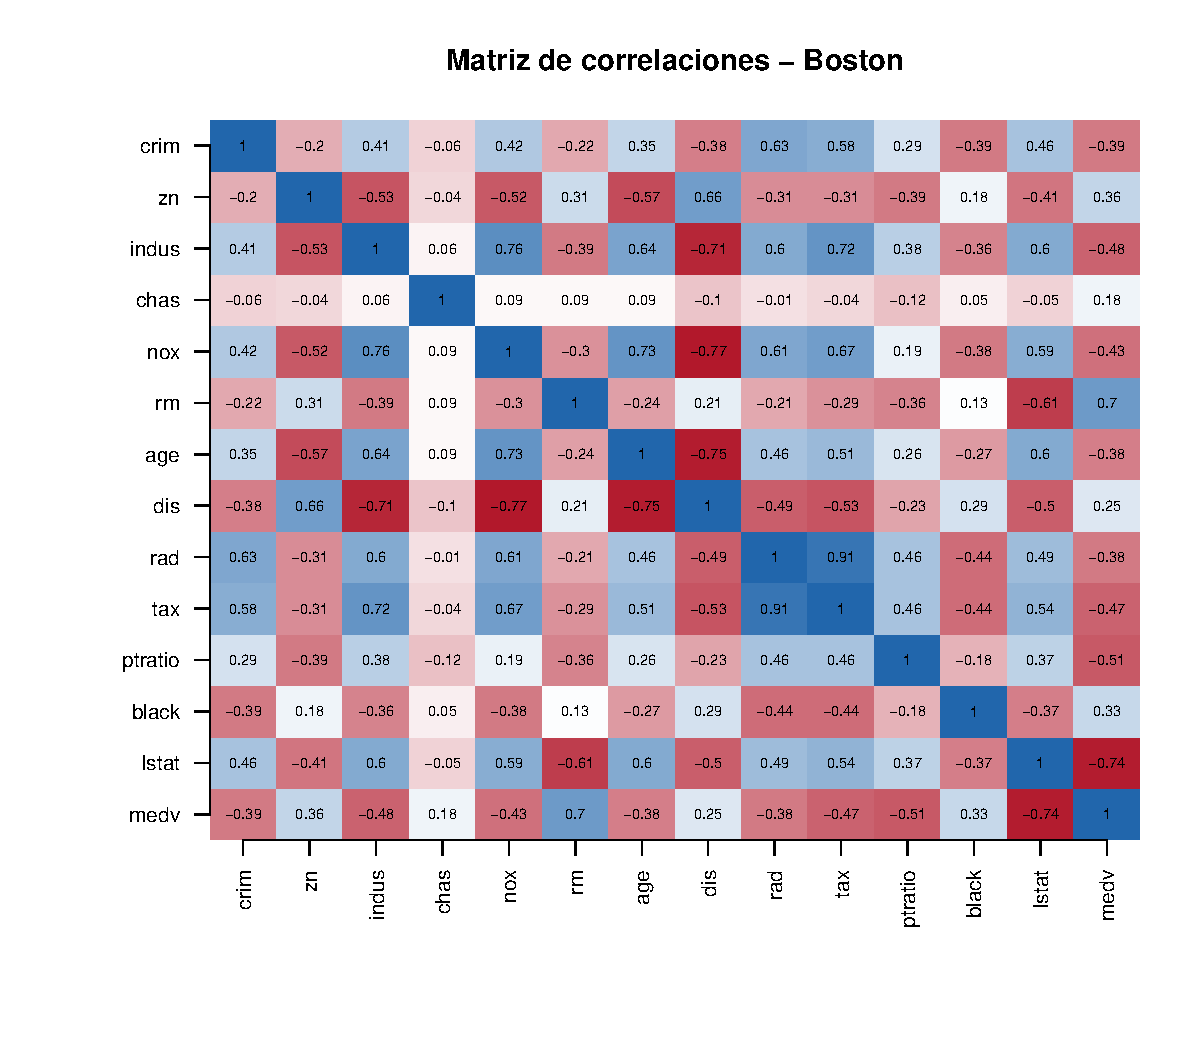
\includegraphics[width=0.72\textwidth]{figuras/fig_01_matriz_correlaciones.pdf}
  \caption{Matriz de correlaciones entre variables del dataset Boston.}
  \label{fig:correlaciones}
\end{figure}

\subsection{Fase 3: Preparacion de los Datos}

Para el PCA exploratorio se seleccionaron las 14 variables originales del dataset: \texttt{crim}, \texttt{zn}, \texttt{indus}, \texttt{chas}, \texttt{nox}, \texttt{rm}, \texttt{age}, \texttt{dis}, \texttt{rad}, \texttt{tax}, \texttt{ptratio}, \texttt{black}, \texttt{lstat} y \texttt{medv}. Se mantuvo \texttt{chas} como variable binaria 0/1, porque indica si el sector limita o no con el rio Charles; no representa una distancia continua. Todas las variables fueron estandarizadas internamente en \texttt{prcomp(center = TRUE, scale. = TRUE)}. La revision previa confirmo medias escaladas cercanas a 0 y desviaciones estandar iguales a 1.

Para la prediccion de criminalidad, \texttt{crim} fue separada como variable objetivo y las restantes variables se usaron como predictores. Por lo tanto, el PCA predictivo no incluye \texttt{crim} como predictor original: primero resume las variables urbanas, socioeconomicas y habitacionales restantes, y despues alimenta una regresion lineal sobre \texttt{log1p(crim)}. Se dividieron los datos en 70\% entrenamiento (354 registros) y 30\% prueba (152 registros), con semilla fija para reproducibilidad.

\subsection{Fase 4: Modelamiento PCA}

El PCA fue aplicado sobre las variables estandarizadas. El primer componente explica 46,76\% de la varianza total, el segundo 11,78\% y el tercero 9,64\%. Los cinco primeros componentes acumulan 80,58\%, por lo que resumen gran parte de la informacion original (Tabla~\ref{tab:pca_varianza}).

\begin{table}[H]
  \centering
  \caption{Varianza explicada por los primeros componentes principales.}
  \label{tab:pca_varianza}
  \footnotesize
  \begin{tabular}{l r r}
    \toprule
    \textbf{Componente} & \textbf{Varianza individual} & \textbf{Varianza acumulada} \\
    \midrule
    PC1 & 46,76\% & 46,76\% \\
    PC2 & 11,78\% & 58,54\% \\
    PC3 & 9,64\% & 68,17\% \\
    PC4 & 6,33\% & 74,51\% \\
    PC5 & 6,08\% & 80,58\% \\
    \bottomrule
  \end{tabular}
\end{table}

La Tabla~\ref{tab:pca_cargas} resume las cargas mas relevantes de PC1 y PC2, tomadas de \texttt{salidas/11\_pca\_cargas\_variables.csv}. PC1 representa principalmente un eje de presion urbana y socioeconomica: las cargas positivas mas altas corresponden a \texttt{indus} (0,3319), \texttt{nox} (0,3252), \texttt{tax} (0,3240), \texttt{lstat} (0,3114) y \texttt{rad} (0,3034), mientras que \texttt{dis} (-0,2982), \texttt{medv} (-0,2666) y \texttt{zn} (-0,2454) se ubican en sentido contrario. Esto indica que los sectores con mayor carga industrial, contaminacion, impuestos, accesibilidad radial y menor estatus socioeconomico se oponen al eje de mayor valor habitacional y mayor suelo residencial.

PC2 funciona como una diferenciacion residencial secundaria. Sus cargas positivas mas altas son \texttt{medv} (0,4449), \texttt{rm} (0,4340) y \texttt{chas} (0,4107), mientras que las negativas principales son \texttt{dis} (-0,3591), \texttt{ptratio} (-0,3146) y \texttt{lstat} (-0,2012). Por ello, PC2 ayuda a conectar el valor de vivienda con mayor numero de habitaciones y con la condicion binaria de limitar con el rio Charles, en oposicion a variables asociadas a distancia a centros de empleo, presion educativa y menor estatus socioeconomico. Esta lectura del biplot permite integrar en una sola vista los patrones que luego se responden con correlaciones, boxplots y regresiones simples.

\begin{table}[H]
  \centering
  \caption{Cargas principales de PC1 y PC2 utilizadas para interpretar el PCA.}
  \label{tab:pca_cargas}
  \footnotesize
  \begin{tabularx}{\textwidth}{l X X X}
    \toprule
    \textbf{Componente} & \textbf{Cargas positivas relevantes} & \textbf{Cargas negativas relevantes} & \textbf{Lectura analitica} \\
    \midrule
    PC1 & \texttt{indus}=0,3319; \texttt{nox}=0,3252; \texttt{tax}=0,3240; \texttt{lstat}=0,3114; \texttt{rad}=0,3034 & \texttt{dis}=-0,2982; \texttt{medv}=-0,2666; \texttt{zn}=-0,2454 & Eje de presion urbana/socioeconomica opuesto al valor habitacional. \\
    PC2 & \texttt{medv}=0,4449; \texttt{rm}=0,4340; \texttt{chas}=0,4107; \texttt{age}=0,2603 & \texttt{dis}=-0,3591; \texttt{ptratio}=-0,3146; \texttt{lstat}=-0,2012 & Eje residencial asociado a precio, habitaciones y limite con el rio Charles. \\
    \bottomrule
  \end{tabularx}
\end{table}

\begin{figure}[H]
  \centering
  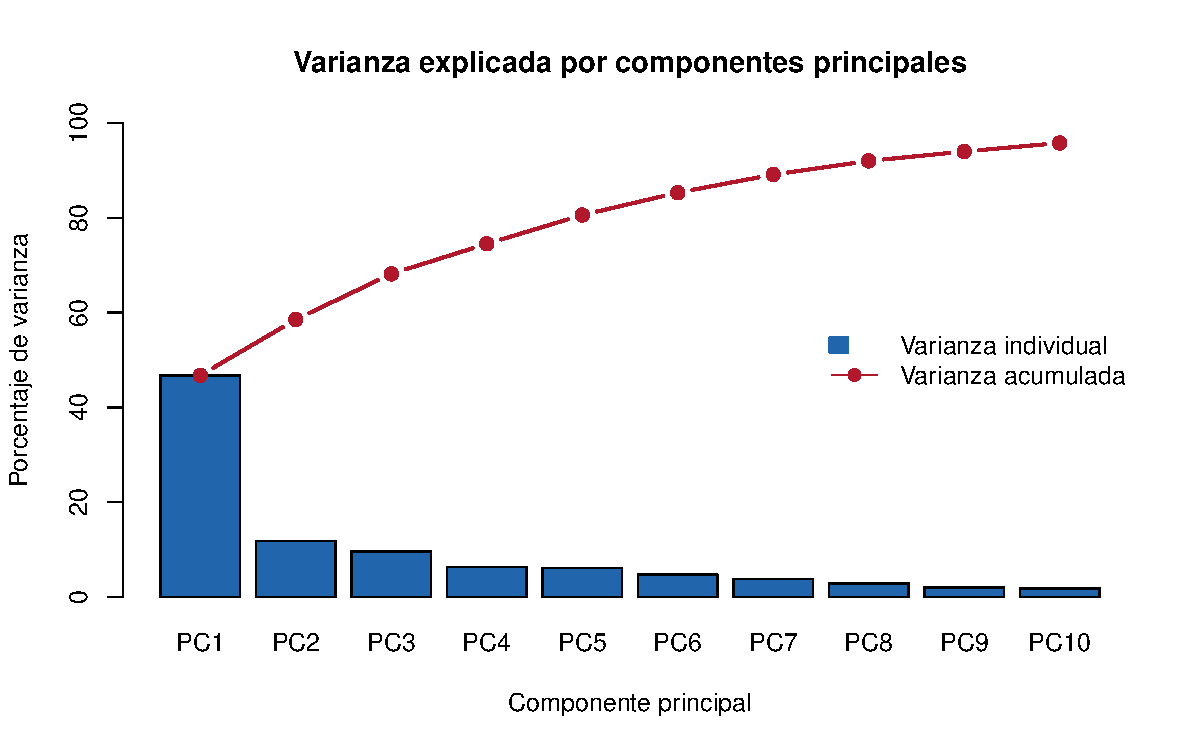
\includegraphics[width=0.70\textwidth]{figuras/fig_07_pca_varianza_explicada.pdf}
  \caption{Varianza individual y acumulada explicada por los componentes principales.}
  \label{fig:pca_varianza}
\end{figure}

\begin{figure}[H]
  \centering
  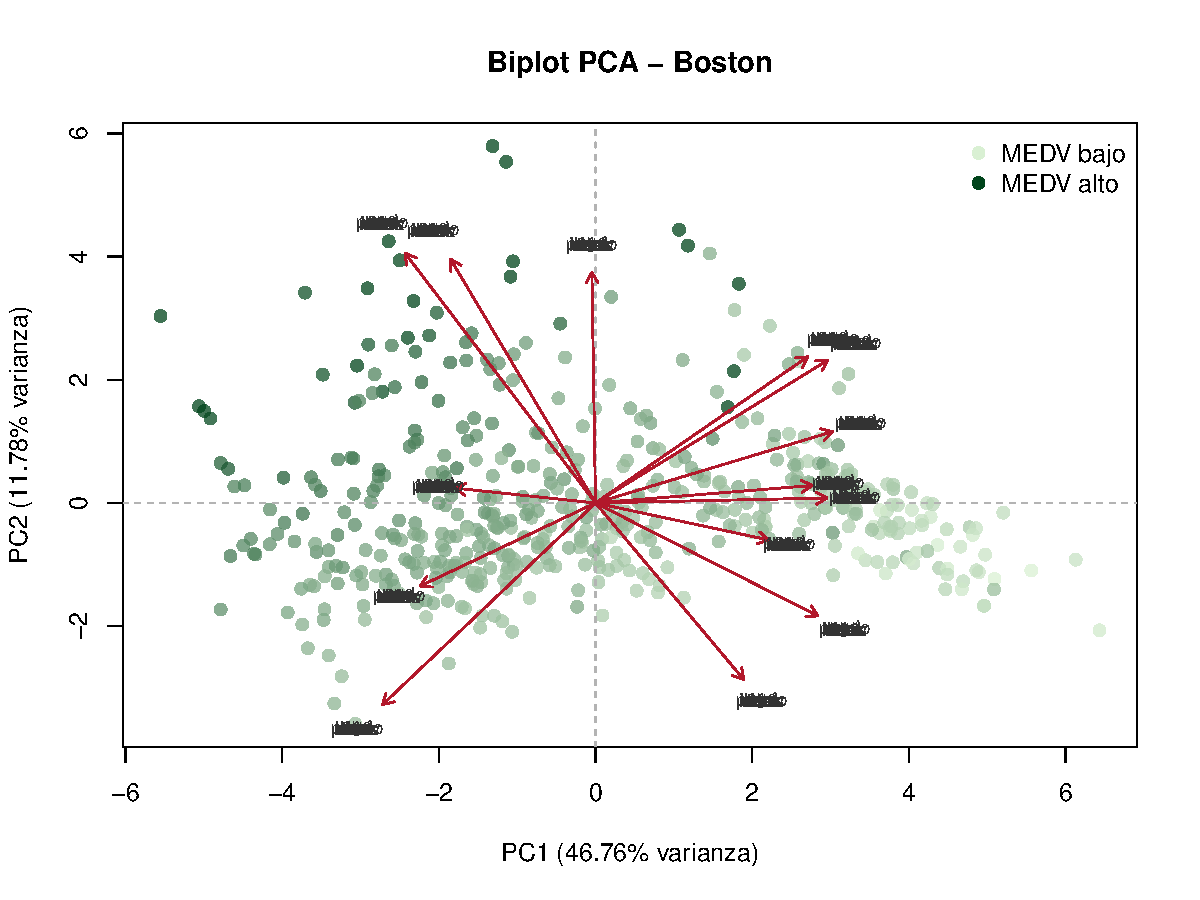
\includegraphics[width=0.78\textwidth]{figuras/fig_08_pca_biplot.pdf}
  \caption{Biplot PCA. Los puntos representan observaciones del dataset y el color indica el valor mediano de vivienda.}
  \label{fig:pca_biplot}
\end{figure}

\subsection{Fase 5: Evaluacion y Respuestas de Investigacion}

\textbf{Pregunta 1: Hay valores atipicos en al menos dos variables?} Si. Usando la regla IQR se detectaron outliers en varias variables. La mayor cantidad aparece en \texttt{black} (77) y \texttt{zn} (68); sin depender de \texttt{black}, tambien destacan \texttt{crim} (66), \texttt{medv} (40) y \texttt{rm} (30), como se observa en la Figura~\ref{fig:outliers}. La lectura PCA ayuda a contextualizar estos outliers: \texttt{crim}, \texttt{zn} y \texttt{medv} tienen cargas relevantes en PC1, mientras que \texttt{rm} y \texttt{medv} tienen alta importancia en PC2. Por tanto, los valores extremos no son solo observaciones aisladas, sino que afectan variables que forman parte de los ejes principales del analisis multivariado. La variable \texttt{black} se reporta por reproducibilidad del dataset, pero no se usa para conclusiones sustantivas por su sensibilidad historica.

\textbf{Pregunta 2: Que suburbios tienen las casas mas baratas?} Dado que el conjunto \texttt{Boston} no incluye nombres de suburbios, se identifican las observaciones del dataset con menor valor mediano de vivienda mediante un identificador interno \texttt{id\_suburbio}. Los registros con menor valor fueron ID 399 y 406, ambos con \texttt{medv = 5}. Luego aparecen ID 401 con 5,6 e ID 400 con 6,3. Todos los diez registros mas baratos no limitan con el rio Charles. En el PCA, \texttt{medv} se opone al eje PC1 de presion urbana (carga -0,2666) y se alinea con PC2 junto con \texttt{rm}; por ello, estas observaciones de bajo precio se interpretan como casos ubicados en la direccion contraria al vector de mayor valor habitacional del biplot.

\textbf{Pregunta 3: Como influye el tamano de la casa en su precio?} La variable \texttt{rm}, numero promedio de habitaciones, presenta una relacion positiva con \texttt{medv}. La correlacion es 0,695 y el modelo lineal \texttt{medv} $\sim$ \texttt{rm} estima que una habitacion promedio adicional se asocia con 9,102 miles de dolares mas en el valor mediano de vivienda ($p < 0,001$). El PCA refuerza esta conclusion: \texttt{rm} (0,4340) y \texttt{medv} (0,4449) tienen cargas positivas muy similares en PC2, por lo que el biplot muestra ambas variables en la misma direccion residencial.

\textbf{Pregunta 4: Afecta la condicion de limitar con el rio Charles al valor de las casas?} Si, con cautela interpretativa. \texttt{chas} es una variable binaria que indica si el sector limita o no con el rio Charles; no mide distancia exacta al rio. Los sectores que no limitan con el rio tienen media \texttt{medv} de 22,094, mientras que los que si limitan tienen media de 28,440. La diferencia media es 6,346 miles de dolares y la prueba t obtiene $p = 0,00357$. En el PCA, \texttt{chas} tiene carga positiva alta en PC2 (0,4107), en la misma direccion que \texttt{medv} (0,4449), lo que respalda multivariadamente la diferencia observada en el boxplot, aunque el grupo con \texttt{chas = 1} solo contiene 35 observaciones.

\textbf{Pregunta 5: Cual es el impacto del estatus socioeconomico?} El impacto es negativo. La correlacion entre \texttt{lstat} y \texttt{medv} es -0,738. El modelo \texttt{medv} $\sim$ \texttt{lstat} estima que cada punto porcentual adicional en \texttt{lstat} se asocia con una disminucion de 0,950 miles de dolares en \texttt{medv} ($p < 0,001$). El PCA confirma esta oposicion: en PC1, \texttt{lstat} carga positivamente (0,3114) y \texttt{medv} negativamente (-0,2666); en PC2, \texttt{medv} carga positivamente (0,4449) y \texttt{lstat} negativamente (-0,2012). Esto muestra que el estatus socioeconomico es un factor estructural en la separacion multivariada del dataset.

\textbf{Pregunta 6: Es posible predecir la tasa de criminalidad?} Si, de forma academica y exploratoria. Para evitar usar \texttt{crim} como predictor de si misma, el PCA predictivo se calculo solo con las variables restantes. Luego se entreno una regresion lineal sobre los primeros 5 componentes principales, que explican 82,84\% de la varianza de los predictores. En prueba se obtuvo $R^2 = 0,8119$ sobre \texttt{log1p(crim)}, RMSE de 7,4102 en escala original y mejora de 11,85\% frente al promedio base. El resultado indica capacidad predictiva razonable porque el PCA resume informacion urbana y socioeconomica relacionada con criminalidad, pero no corresponde a un modelo listo para despliegue.

\begin{figure}[H]
  \centering
  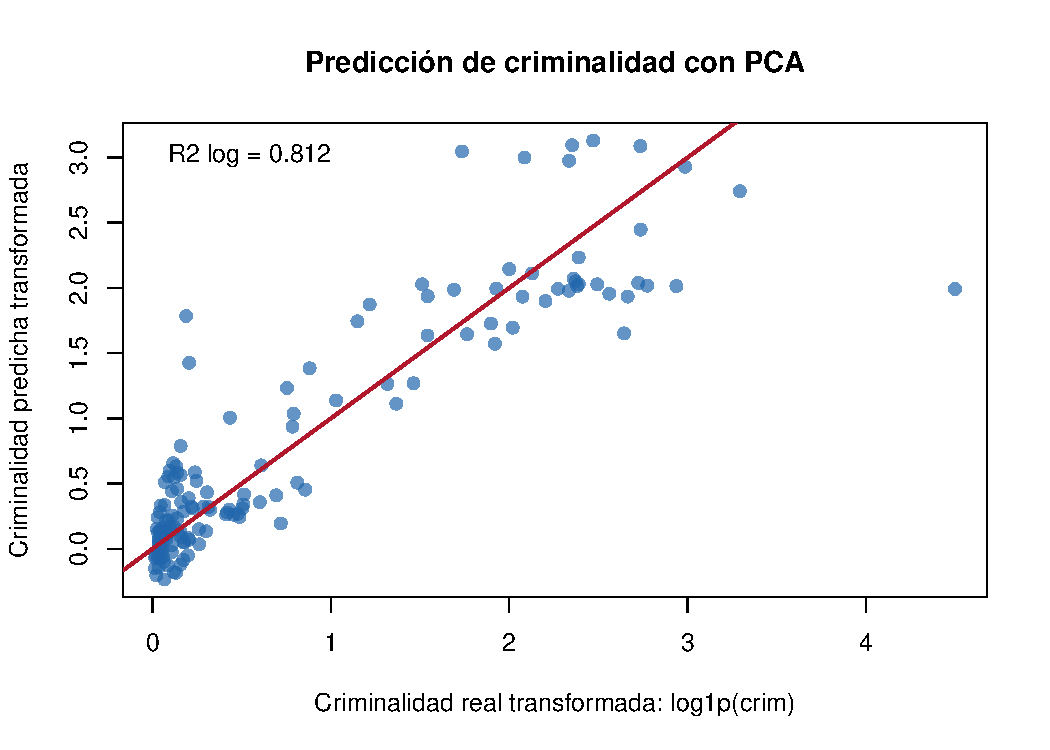
\includegraphics[width=0.70\textwidth]{figuras/fig_09_prediccion_crim.pdf}
  \caption{Prediccion de criminalidad transformada mediante regresion sobre componentes principales.}
  \label{fig:prediccion_crim}
\end{figure}

La Tabla~\ref{tab:resumen_preguntas} sintetiza la evaluacion final de CRISP-DM: cada pregunta fue respondida con una tecnica especifica y, cuando corresponde, conectada con la estructura multivariada del PCA. Esta integracion evita que el PCA quede como una visualizacion aislada y lo posiciona como el eje que resume los patrones encontrados en las fases exploratorias.

\begin{table}[H]
  \centering
  \caption{Resumen de preguntas, evidencias y relacion con PCA.}
  \label{tab:resumen_preguntas}
  \footnotesize
  \begin{tabularx}{\textwidth}{p{2.2cm} X X}
    \toprule
    \textbf{Pregunta} & \textbf{Tecnica directa} & \textbf{Aporte del PCA} \\
    \midrule
    P1 Outliers & Regla IQR sobre variables numericas. & Variables con outliers como \texttt{crim}, \texttt{zn}, \texttt{medv} y \texttt{rm} participan en PC1 o PC2. \\
    P2 Baratas & Ordenamiento ascendente por \texttt{medv}. & \texttt{medv} define una direccion relevante del biplot y se opone al eje PC1 de presion urbana. \\
    P3 Tamano & Correlacion y regresion \texttt{medv} $\sim$ \texttt{rm}. & \texttt{rm} y \texttt{medv} cargan positivamente y en la misma direccion en PC2. \\
    P4 Rio Charles & Comparacion de medias y prueba t segun \texttt{chas}. & \texttt{chas} carga positivamente en PC2 junto con \texttt{medv}; se interpreta como variable binaria. \\
    P5 Estatus & Correlacion y regresion \texttt{medv} $\sim$ \texttt{lstat}. & \texttt{lstat} y \texttt{medv} aparecen en direcciones opuestas en PC1 y PC2. \\
    P6 Criminalidad & Regresion sobre componentes principales para \texttt{log1p(crim)}. & El PCA reduce dimensionalidad de predictores sin incluir \texttt{crim}. \\
    \bottomrule
  \end{tabularx}
\end{table}

\section{Discusion y Reflexion}

La metodologia CRISP-DM permitio ordenar el trabajo desde la definicion de preguntas hasta la evaluacion del modelo. El PCA fue util porque el dataset contiene variables altamente relacionadas: zonas con mayor industrializacion, contaminacion, accesibilidad radial, impuestos y menor estatus socioeconomico tienden a agruparse en la misma direccion del PC1, mientras que el valor habitacional se orienta en sentido contrario. Esto aporta una lectura multivariada mas clara que analizar cada variable de forma aislada.

Los resultados sobre precio son consistentes: mas habitaciones se asocian con mayor valor, mientras que mayor porcentaje de poblacion de menor estatus socioeconomico se asocia con menor valor. La condicion de limitar con el rio Charles tambien muestra una diferencia positiva en promedio, pero debe interpretarse con cautela porque \texttt{chas} no mide distancia exacta y solo 35 de 506 observaciones limitan con el rio.

La prediccion de criminalidad mejora al usar componentes principales, especialmente al transformar la variable objetivo con \texttt{log1p}. La ventaja metodologica es que los componentes sintetizan informacion urbana y socioeconomica antes de la regresion, reduciendo redundancia entre predictores. Sin embargo, la existencia de valores extremos en \texttt{crim}, el caracter historico del dataset y la sensibilidad de algunas variables limitan la generalizacion. Para una aplicacion real seria necesario validar con datos actuales, revisar sesgos, evaluar modelos no lineales y considerar implicancias eticas.

\section{Conclusiones}

\textbf{Vicente Rivera:} El analisis exploratorio mostro ausencia de valores faltantes, pero presencia importante de outliers en \texttt{black} (77), \texttt{zn} (68), \texttt{crim} (66), \texttt{medv} (40) y \texttt{rm} (30). Para evitar una conclusion dependiente de \texttt{black}, se considero especialmente \texttt{zn} y \texttt{crim}. Estas variables tambien participan en la estructura PCA, lo que confirma que los valores extremos afectan dimensiones relevantes del caso.

\textbf{Juan Mu\~noz:} La aplicacion de CRISP-DM permitio estructurar el analisis de manera clara. El PCA resumio el 80,58\% de la varianza en cinco componentes; PC1 agrupo variables de presion urbana como \texttt{indus}, \texttt{nox}, \texttt{tax}, \texttt{lstat} y \texttt{rad}, mientras que \texttt{medv} se ubico en sentido contrario. Esto respalda que mayor presion urbana y socioeconomica se asocia con menor valor habitacional.

\textbf{Fernando Valdes:} La implementacion en R fue reproducible y simple. La relacion positiva entre \texttt{rm} y \texttt{medv} se observo tanto en la regresion (pendiente 9,102) como en PC2, donde ambas variables cargan positivamente. La regresion con componentes principales alcanzo $R^2 = 0,8119$ en escala logaritmica para criminalidad, lo que muestra utilidad predictiva exploratoria, aunque no suficiente para uso operativo sin validacion adicional.

\section{Referencias}
\small
\begin{thebibliography}{9}

\bibitem[Chapman et~al.(2000)]{chapman2000}
Chapman, P., Clinton, J., Kerber, R., Khabaza, T., Reinartz, T., Shearer, C., y Wirth, R. (2000).
\textit{CRISP-DM 1.0: Step-by-step data mining guide}. SPSS Inc.

\bibitem[Harrison y Rubinfeld(1978)]{harrison1978}
Harrison, D., y Rubinfeld, D. L. (1978).
Hedonic housing prices and the demand for clean air.
\textit{Journal of Environmental Economics and Management}, 5(1), 81--102.

\bibitem[Jolliffe(2002)]{jolliffe2002}
Jolliffe, I. T. (2002).
\textit{Principal Component Analysis} (2nd ed.). Springer.

\bibitem[R Core Team(2024)]{rcore2024}
R Core Team. (2024).
\textit{R: A Language and Environment for Statistical Computing}. R Foundation for Statistical Computing.
\url{https://www.R-project.org/}

\bibitem[Venables y Ripley(2002)]{venables2002}
Venables, W. N., y Ripley, B. D. (2002).
\textit{Modern Applied Statistics with S} (4th ed.). Springer.

\end{thebibliography}

\newpage
\section*{Anexo}
\addcontentsline{toc}{section}{Anexo}

\subsection*{A.1 Visualizaciones Complementarias}

\begin{figure}[H]
\centering
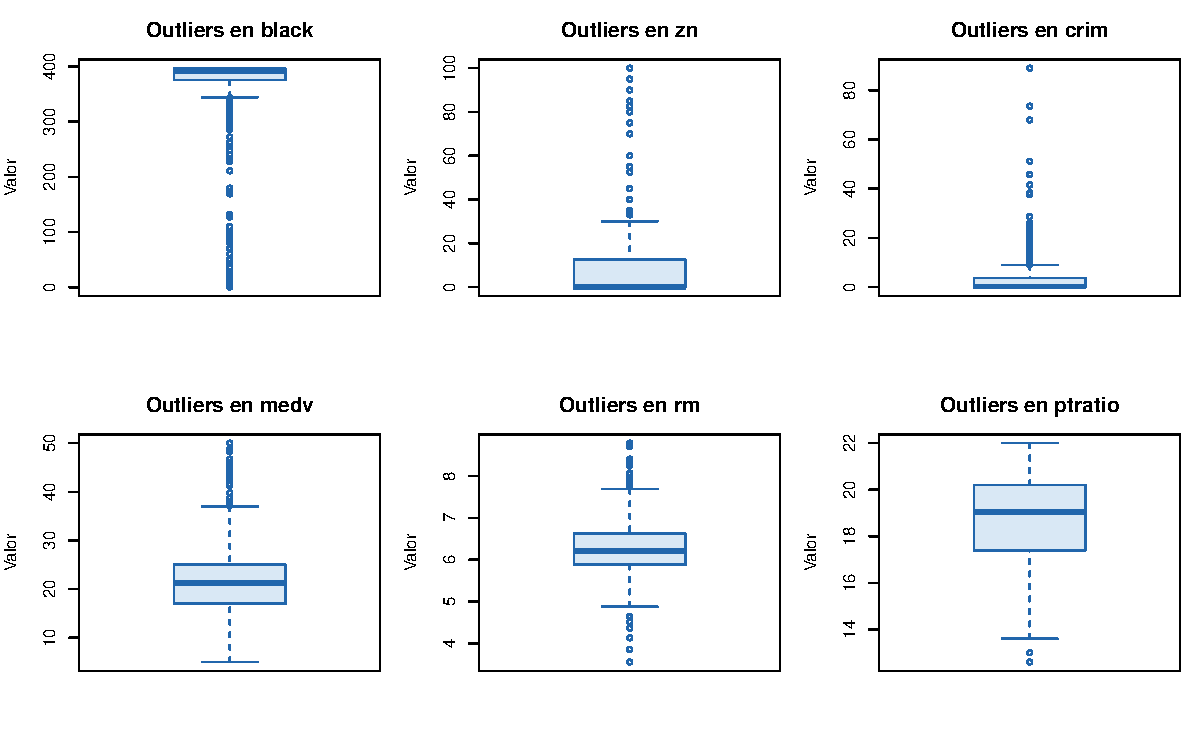
\includegraphics[width=0.85\textwidth]{figuras/fig_02_outliers_boxplot.pdf}
\caption{Variables con mayor cantidad de valores atipicos segun regla IQR.}
\label{fig:outliers}
\end{figure}

\begin{figure}[H]
\centering
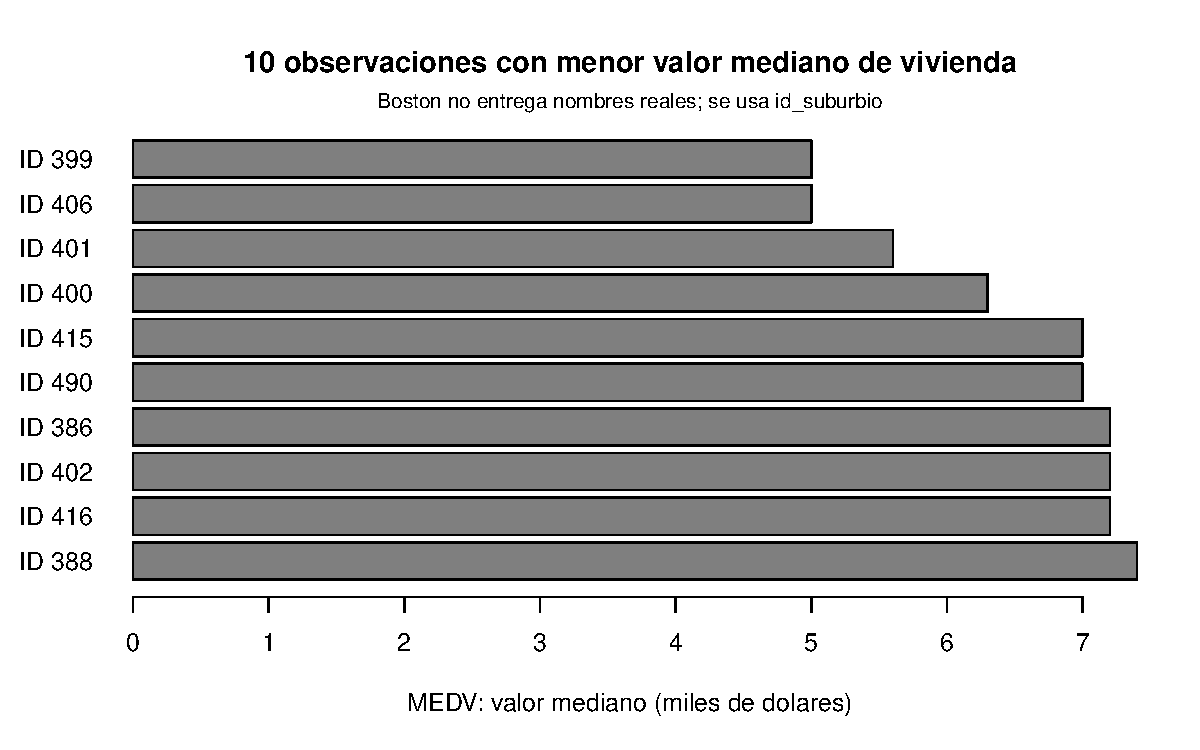
\includegraphics[width=0.82\textwidth]{figuras/fig_03_suburbios_mas_baratos.pdf}
\caption{Diez observaciones del dataset con menor valor mediano de vivienda.}
\label{fig:baratos}
\end{figure}

\begin{figure}[H]
\centering
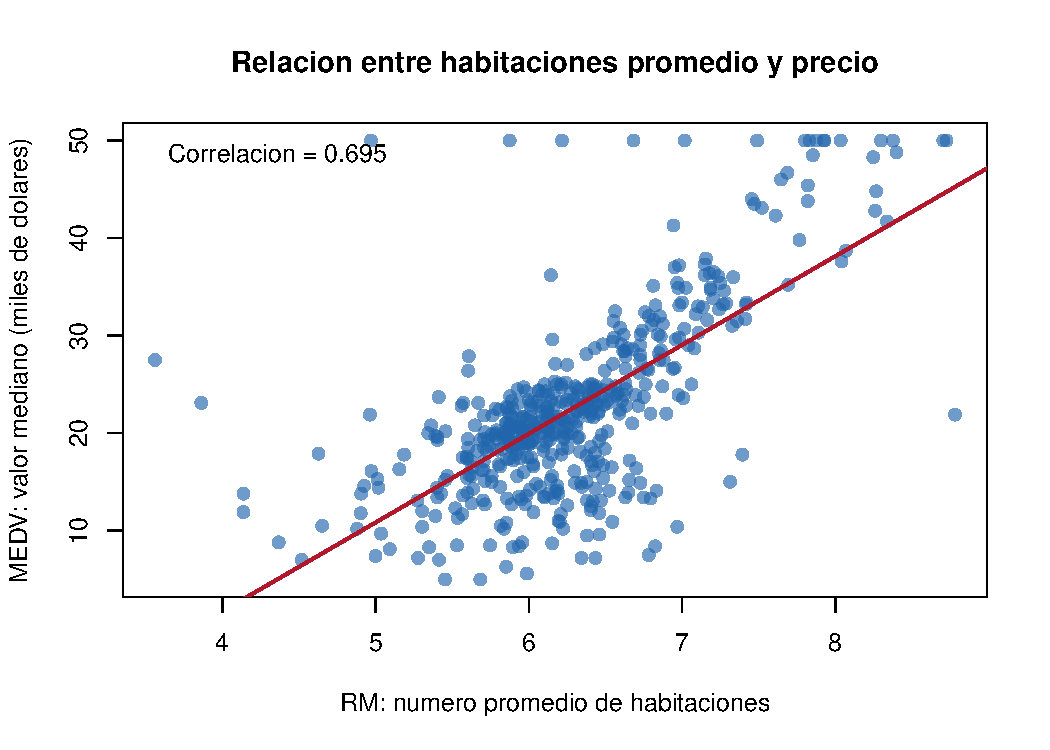
\includegraphics[width=0.72\textwidth]{figuras/fig_04_rm_vs_medv.pdf}
\caption{Relacion entre habitaciones promedio y valor mediano de vivienda.}
\label{fig:rm_medv}
\end{figure}

\begin{figure}[H]
\centering
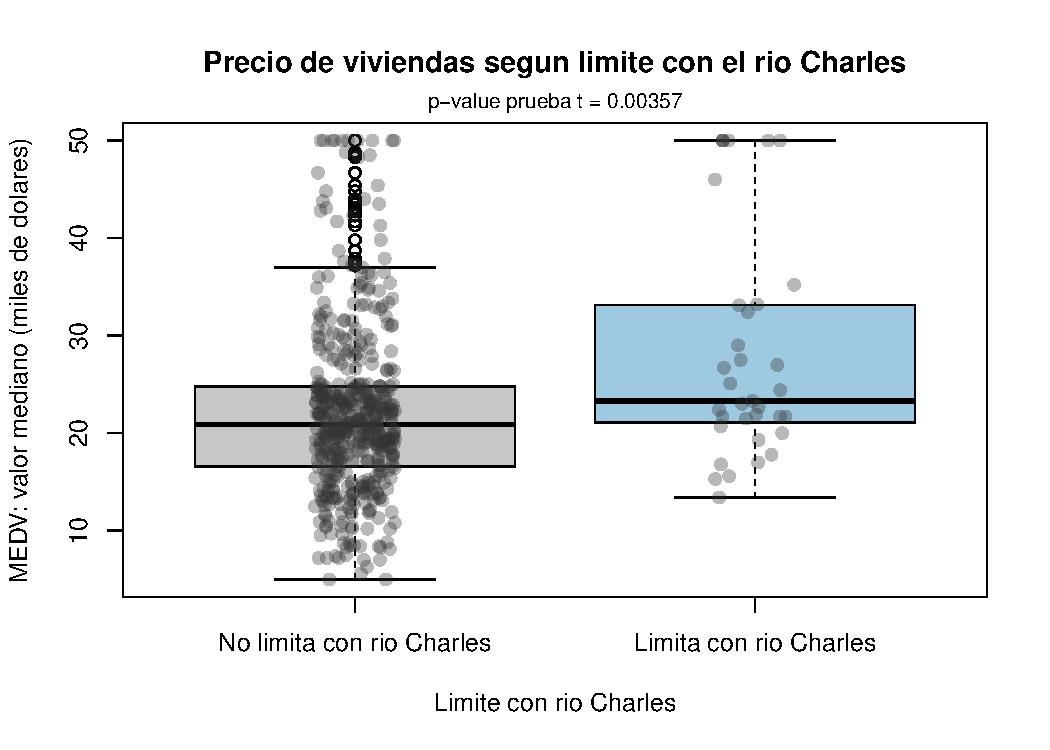
\includegraphics[width=0.72\textwidth]{figuras/fig_05_chas_vs_medv.pdf}
\caption{Valor mediano de viviendas segun limite con el rio Charles.}
\label{fig:chas_medv}
\end{figure}

\begin{figure}[H]
\centering
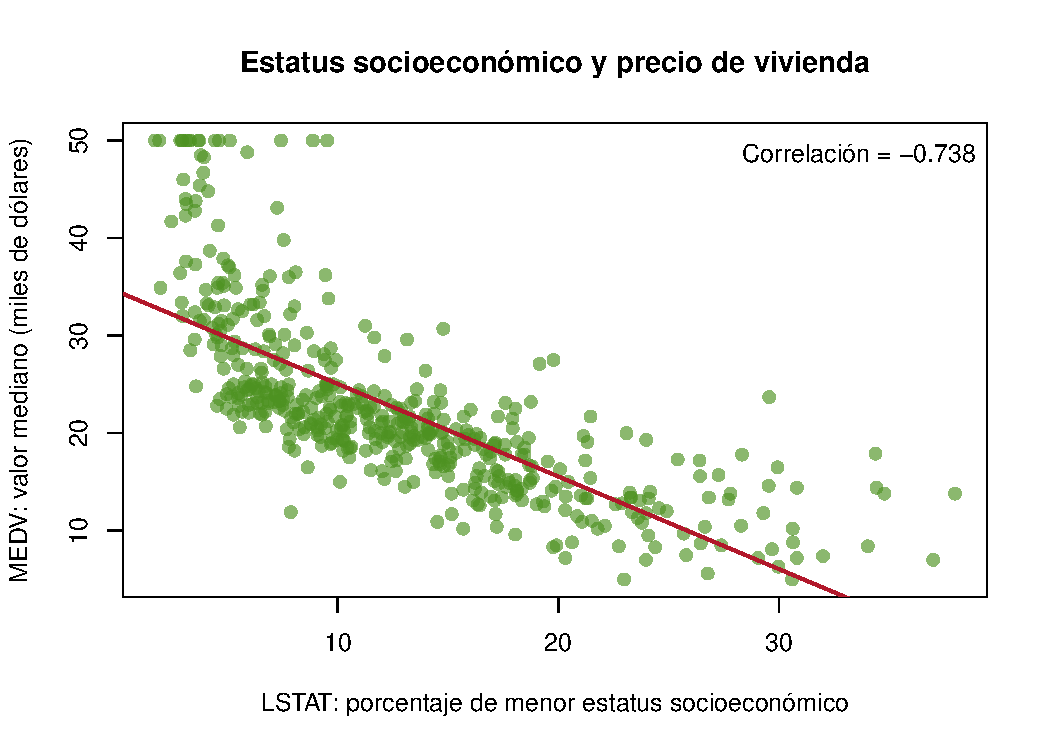
\includegraphics[width=0.72\textwidth]{figuras/fig_06_lstat_vs_medv.pdf}
\caption{Relacion entre estatus socioeconomico y valor mediano de vivienda.}
\label{fig:lstat_medv}
\end{figure}

\subsection*{A.2 Procedimientos Principales en R}

El codigo completo se encuentra en el archivo \texttt{tarea4\_boston\_pca.R}. A continuacion se muestran los procedimientos principales.

\begin{lstlisting}[caption={Carga de datos y revision inicial.}]
library(MASS)
data("Boston", package = "MASS")

boston <- Boston
boston$id_suburbio <- seq_len(nrow(boston))
boston$chas_factor <- factor(boston$chas,
  levels = c(0, 1),
  labels = c("No limita con rio Charles",
             "Limita con rio Charles"))

summary(boston)
colSums(is.na(boston))
\end{lstlisting}

\begin{lstlisting}[caption={PCA sobre variables estandarizadas.}]
vars_analisis <- c("crim", "zn", "indus", "chas", "nox", "rm",
  "age", "dis", "rad", "tax", "ptratio", "black", "lstat", "medv")

pca_data <- boston[, vars_analisis]
pca_boston <- prcomp(pca_data, center = TRUE, scale. = TRUE)

varianza <- pca_boston$sdev^2 / sum(pca_boston$sdev^2)
round(cumsum(varianza) * 100, 2)

cargas <- as.data.frame(pca_boston$rotation[, 1:2])
cargas$abs_PC1 <- abs(cargas$PC1)
cargas$abs_PC2 <- abs(cargas$PC2)
cargas[order(-cargas$abs_PC1), ]
\end{lstlisting}

\begin{lstlisting}[caption={Prediccion de criminalidad con componentes principales.}]
vars_predictoras_crim <- setdiff(vars_analisis, "crim")
idx_train <- sample(seq_len(nrow(boston)), size = floor(0.70 * nrow(boston)))

train <- boston[idx_train, c("crim", vars_predictoras_crim)]
test <- boston[-idx_train, c("crim", vars_predictoras_crim)]

pca_pred <- prcomp(train[, vars_predictoras_crim],
                  center = TRUE, scale. = TRUE)

varianza_pred <- pca_pred$sdev^2 / sum(pca_pred$sdev^2)
n_componentes <- which(cumsum(varianza_pred) >= 0.80)[1]
pc_modelo <- paste0("PC", seq_len(n_componentes))

train_pcs <- as.data.frame(pca_pred$x[, pc_modelo, drop = FALSE])
train_pcs$log_crim <- log1p(train$crim)

test_pcs <- as.data.frame(
  predict(pca_pred, newdata = test[, vars_predictoras_crim])[, pc_modelo]
)

modelo_crim <- lm(log_crim ~ ., data = train_pcs)
pred_log_crim <- predict(modelo_crim, newdata = test_pcs)
\end{lstlisting}

\subsection*{A.3 Bitacora de Trabajo}

\begin{table}[H]
  \centering
  \footnotesize
  \caption{Bitacora de trabajo grupal.}
  \label{tab:bitacora}
  \begin{tabularx}{\textwidth}{l X l}
    \toprule
    \textbf{Fecha} & \textbf{Actividad} & \textbf{Responsable} \\
    \midrule
    Dia 1 & Lectura del enunciado, definicion de preguntas de investigacion y revision de la metodologia CRISP-DM. & Todos \\
    Dia 2 & Carga del dataset Boston, revision de estructura, resumen estadistico, valores faltantes y matriz de correlaciones. & Vicente Rivera \\
    Dia 3 & Deteccion de valores atipicos, analisis de observaciones con menor valor y modelos simples para \texttt{rm}, \texttt{chas} y \texttt{lstat}. & Juan Mu\~noz \\
    Dia 4 & Preparacion de variables, estandarizacion y aplicacion de PCA con interpretacion de varianza y cargas. & Fernando Valdes \\
    Dia 5 & Modelamiento predictivo de criminalidad usando componentes principales y evaluacion con RMSE, MAE y $R^2$. & Todos \\
    Dia 6 & Redaccion del informe en LaTeX, integracion de figuras, revision de resultados y preparacion de entrega. & Todos \\
    \bottomrule
  \end{tabularx}
\end{table}

\end{document}
